\documentclass{homework}

\linespread{1.2}

\usepackage[T1]{fontenc}\usepackage{palatino}
\usepackage{amssymb,amsmath,amsthm,mathtools}
\usepackage[english]{babel}
\usepackage[utf8]{inputenc}
\usepackage[babel]{csquotes}
\usepackage[pdftex]{hyperref}
\usepackage{enumitem}
\usepackage[usenames,dvipsnames,table,xcdraw]{xcolor}

\usepackage{graphicx} 
\usepackage{verbatim} % Commenti in blocco con \begin{comment}
\usepackage{bm}
\usepackage[font={small,it}]{caption}
\usepackage{subcaption}
\usepackage{geometry}
\usepackage{array}
\usepackage{enumitem}
\setlist[enumerate]{label*=\arabic*.}
	
\usepackage{algorithm}
\usepackage[noend]{algpseudocode}
\usepackage{listings}

\definecolor{mygraybackground}{gray}{0.95}

% Define the R listings to write code
\lstset{
  language=R,
  basicstyle=\scriptsize\ttfamily, 
  numbers=left,
  numberstyle=\small\ttfamily\color{Gray},
  numbersep=10pt,
  backgroundcolor=\color{mygraybackground},
  showstringspaces=false,
  showtabs=false,
  tabsize=3,
  breaklines=true,
  captionpos=b,   
  keywordstyle=\color{black},
  commentstyle=\color{ForestGreen},
}

\makeatletter
\def\BState{\State\hskip-\ALG@thistlm}
\makeatother

% Simbolo iid
\newcommand\iid{\stackrel{\mathclap{\normalfont\tiny\mbox{iid}}}{\sim}}
% Simbolo ind
\newcommand\ind{\stackrel{\mathclap{\normalfont\tiny\mbox{ind}}}{\sim}}

\title{SDS 385: Homework 1}
\author{G.~Paulon}

\begin{document}

\makeatletter
\begin{titlepage}
	\vspace*{\fill}
	\centering
	{\huge \@title \par}
	\vskip0.5cm
	{\large \@author \par}
	\vskip0.5cm
	{\large \today \par}
	\vspace*{\fill}
\end{titlepage}
\makeatother

\newpage 
\mbox{}
\thispagestyle{empty}
\newpage

\setcounter{page}{1}

\problem{Linear regression}

\begin{enumerate}[label=(\Alph*)]
\item Let us write the WLS objective (or cost) function $$l (\beta) = \sum_{i=1}^N \frac{w_i}{2} (y_i - x_i^T \beta)^2$$ in a matricial form. We get 
\begin{align*}
l(\beta) &= \frac{1}{2} (y - X \beta)^T W (y - X \beta)
\\
&= \frac{1}{2} (y^T - (X \beta)^T) W (y - X \beta)
\\
&= \frac{1}{2} \left( y^T W y - y^T W X \beta - (X \beta)^T W y + (X \beta)^T W X \beta \right) 
\end{align*}
Let us remark here that the second and the third term of the sum can be collected in one single term. In fact 
$$(y^T W X \beta)^T = (X \beta)^T W y,$$ i.e. the first is the transposed of the second but, since they are real numbers, they are also equal. Hence we have
\begin{equation*}
l(\beta) = \frac{1}{2} \left( y^T W y - 2 \beta^T X^T W y + \beta^T X^T W X \beta \right). 
\end{equation*}

Since we are trying to minimize a convex function, we can just find its stationary points. To do this, we first need to calculate the gradient of the WLS objective function equalizing it to $0$. Thus, 
\begin{align*}
&\nabla l (\hat{\beta}) = 0
\\
\Leftrightarrow &\frac{1}{2} (- 2 X^T W y + 2 X^T W X \hat{\beta}) = 0
\\
\Leftrightarrow &(X^T W X) \hat{\beta} = X^T W y,
\end{align*}
which is the set of desired equations (also known as normal equations). 

\item Solving the linear system requires the matrix $X^T W X$ to be nonsingular (and therefore invertible). The matrix $X^T W X$ is positive definite, and therefore nonsingular, in case $X$ has full rank (i.e. the columns of $X$ are linearly independent). The normal equations can be easily solved by inverting the matrices, which leads to
$$\hat{\beta} = (X^T W X)^{-1} X^T W y.$$
The classical inversion method, however, is not recommended as its computational complexity grows rapidly as the dimension of the matrices increases. Moreover, the inversion of a matrix is not stable numerically speaking, as small perturbations on the original matrix can produce high differences in the inverse matrices (i.e. the numerical solution does not approach the exact one).

For these reasons, we present here two other approaches that are used to deal with the solution of linear systems: the QR and the Cholesky factorizations. 
\begin{itemize}
\item The QR factorization consists in finding two matrices $Q$ (orthogonal) and $R$ (upper triangular) such that a matrix $A$ can be written as their product. In our case, we want to write the QR factorization of $W^{\frac{1}{2}}X$, i.e. $W^{\frac{1}{2}}X = QR$. Therefore we get 
\begin{align*}
&(X^T W X) \hat{\beta} = X^T W y 
\\
\Leftrightarrow & (W^\frac{1}{2} X)^T (W^\frac{1}{2} X) \hat{\beta} = (W^\frac{1}{2} X)^T W^\frac{1}{2} y
\\
\Leftrightarrow & (QR)^T QR \hat{\beta} = (QR)^T W^\frac{1}{2} y
\\
\Leftrightarrow & R^T Q^T Q R \hat{\beta} = R^T Q^T W^\frac{1}{2} y
\\
\Leftrightarrow & R \hat{\beta} = Q^T W^\frac{1}{2} y.
\end{align*}
This system can be easily solved because $R$ is upper triangular.

In our case, the pseudocode can be summarized as follows.
\begin{algorithm}
\caption{QR solver}\label{alg:qr}
\begin{algorithmic}[1]
\Procedure{My\_QR}{X, y, W}
\State find the factors $Q, R$, s.t. $W^\frac{1}{2} X = QR$
\State compute the right-term: $b \gets Q^T W^{\frac{1}{2}} y$
\State solve the linear system: $\hat{\beta} \gets R^{-1} b$
\EndProcedure
\end{algorithmic}
\end{algorithm}

\item The Cholesky factorization can be found for symmetric and positive definite matrices, and it consists in factorizing the original matrix as $A = RR^T$, where $R$ is a lower triangular matrix. 

In our case, the pseudocode can be summarized as follows.
\begin{algorithm}
\caption{Cholesky solver}\label{alg:chol}
\begin{algorithmic}[1]
\Procedure{My\_Chol}{X, y, W}
\State find the factor $R$, s.t. $X^TWX = RR^T$
\State solve the first linear system: $q \gets R^{-1} X^TWy$
\State solve the second linear system: $\hat{\beta} \gets R^{-T} q$
\EndProcedure
\end{algorithmic}
\end{algorithm}
\end{itemize}

\item We here compare the three methods used to solve the linear system of the normal equations. Let us point out that in each of the three algorithms we exploited the fact that $W$ is a diagonal matrix, optimizing the matricial product $X^TW$ by simply multiplying the first element of the diagonal of $W$ by the first column of $X^T$, and so on. Moreover, since the matrix $X^T W X$ is symmetric, one can exploit this information to calculate it by using R's $\texttt{crossprod} (W^\frac{1}{2} X)$ function.

The performances of the three algorithms are displayed in Figure \ref{fig:perf1}. Four test cases were analysed: the values of $N$ and $P$ range from a minimum of $(N,P) = (100,10)$ to a maximum of $(N,P) = (3000,1000)$. As one can see, Cholesky method is the fastest one. The inversion is slower than Cholesky method and it is also more unstable than every other method, and therefore it has to be avoided. The QR factorization, despite being the slowest method, is preferable when numerical issues can occur. In fact, this method is the most robust one.

\begin{figure}[!ht]
\centering
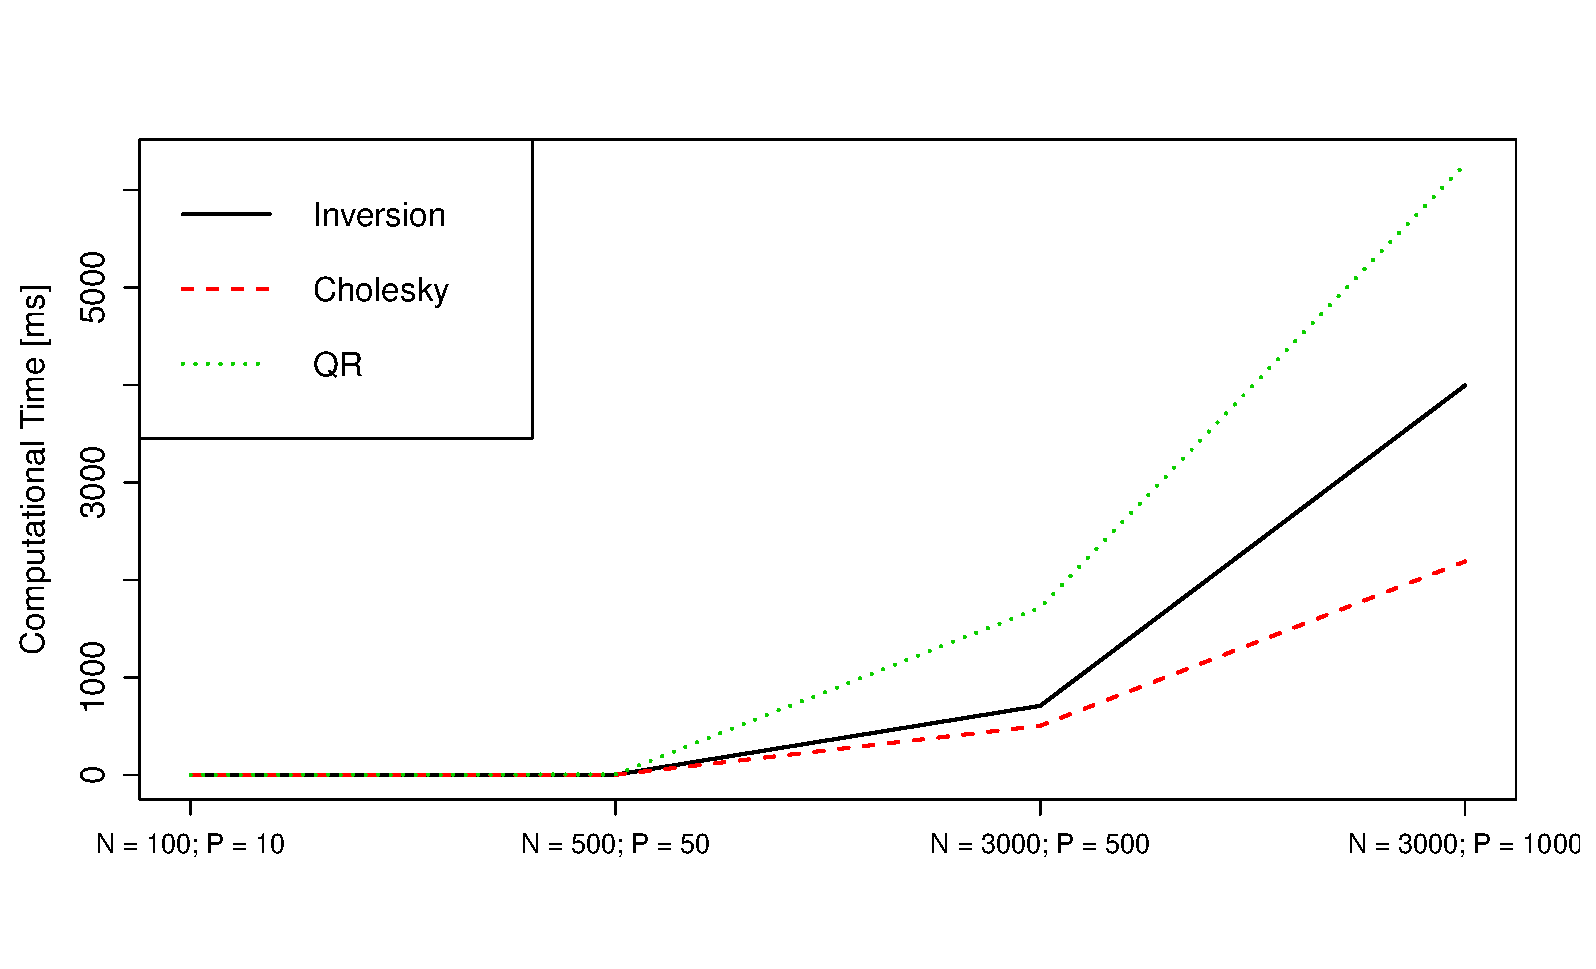
\includegraphics[width=0.6\columnwidth]{./Img/perf}
\caption{Comparison between the performances of the three algorithms for different dimensions of the data and of their features.}
\label{fig:perf1}
\end{figure}

\item In the following we use Cholesky method instead of the QR factorization, as the first is faster and now the primary interest is the performance of the algorithms. If $X$ is a highly sparse matrix, one can exploit appropriate routines in R language in order to make the computation faster. 

\begin{figure}[!ht]
\centering
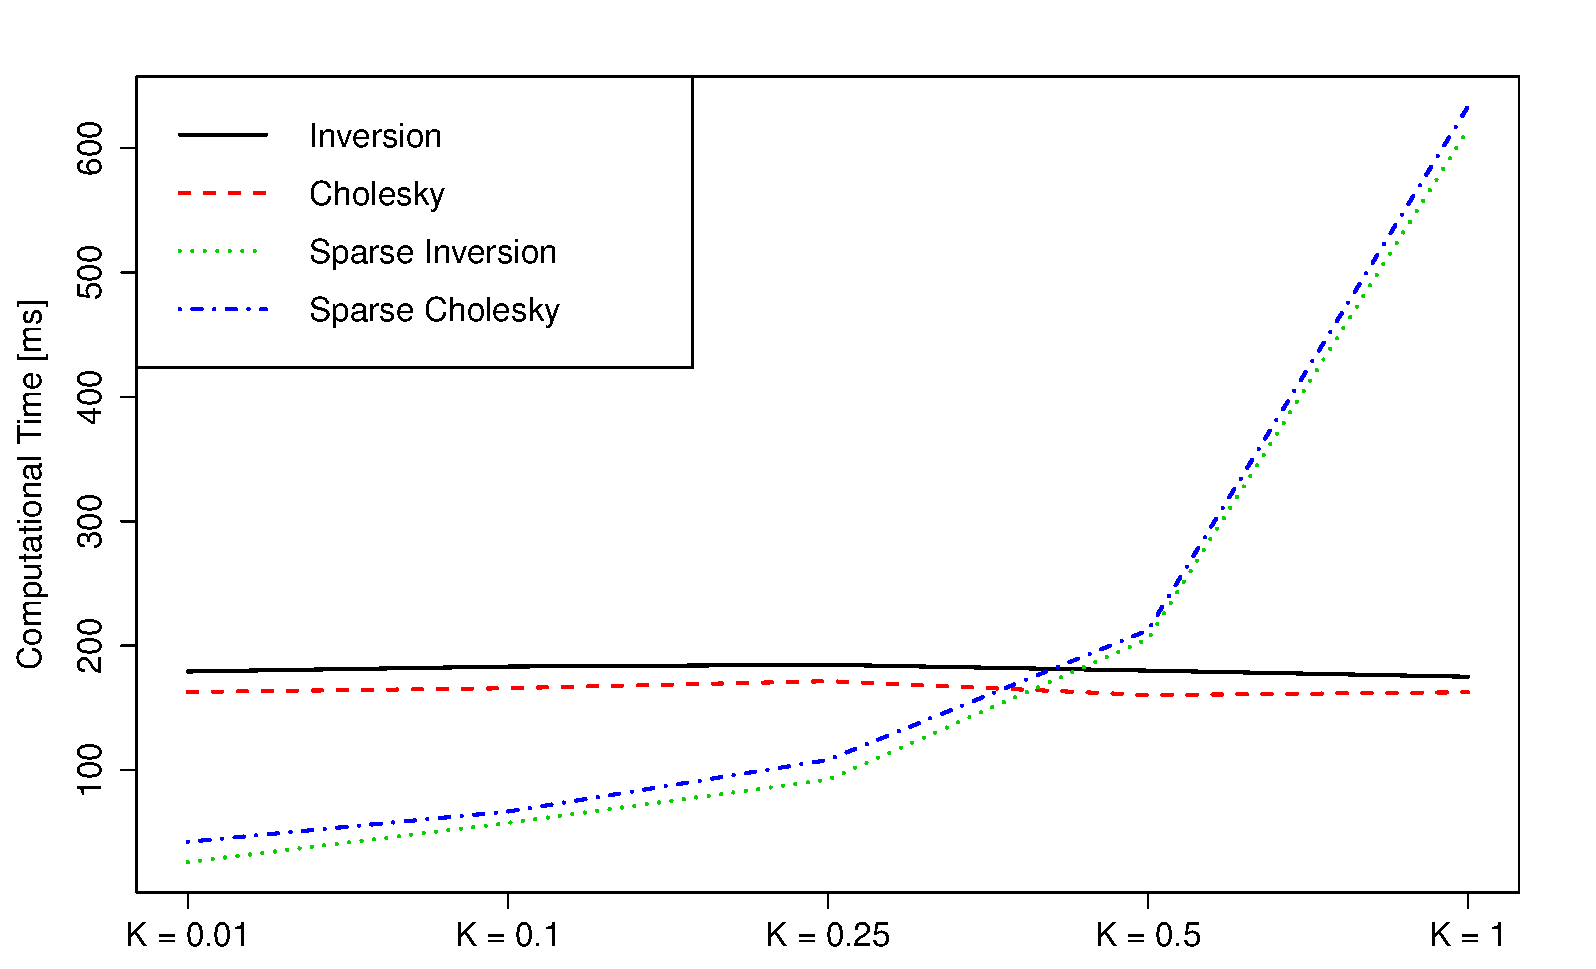
\includegraphics[width=0.6\columnwidth]{./Img/perf_2}
\caption{Comparison between the performances of the three algorithms for different sparsity levels $K$.}
\label{fig:perf2}
\end{figure}

Let us take, as an example, $(N, P) = (1000,500)$ and let us compare the results for different levels of sparsity $K$ of the matrix $X$. As one can see in Figure \ref{fig:perf2}, when the features matrix is dense, both the Cholesky and the inversion methods outperform the sparse method, as this latter involves a first stage in which $X$ is converted in a sparse format. However, as $K$ increases, the sparse method becomes significantly faster than the others. This is due to the fact that matricial products are more efficient in a sparse format and a lot of useless computations is avoided.

\end{enumerate}

\problem{Generalized linear models}

\begin{enumerate}[label=(\Alph*)]
\item The negative log-likelihood for the problem of logistic regression can be written as
\begin{align*}
l(\beta) &= - \log\left\lbrace \prod_{i=1}^N p(y_i | \beta) \right\rbrace
\\
&= -\sum_{i=1}^N \left\lbrace \log \binom{m_i}{y_i} + y_i \log(w_i) + (m_i - y_i) \log (1 - w_i) \right\rbrace.
\end{align*}
The gradient of this latter expression is 
\begin{align*}
\nabla l(\beta) &= - \sum_{i=1}^N \left\lbrace y_i \frac{1}{w_i} \frac{x_i e^{-x_i^T \beta}}{(1+e^{-x_i^T \beta})^2} - (m_i - y_i) \frac{1}{1-w_i} \frac{x_i e^{-x_i^T \beta}}{(1+e^{-x_i^T \beta})^2} \right\rbrace
\\
&= - \sum_{i=1}^N \left\lbrace y_i \frac{x_i e^{-x_i^T \beta}}{1+e^{-x_i^T \beta}} - m_i \frac{x_i}{1+e^{-x_i^T \beta}} + y_i \frac{x_i}{1+e^{-x_i^T \beta}} \right\rbrace
\\
&= - \sum_{i=1}^N \left\lbrace y_i x_i - m_i \frac{x_i}{1+e^{-x_i^T \beta}} \right\rbrace
\\
&= - \sum_{i=1}^N \left\lbrace x_i (y_i - m_i w_i) \right\rbrace
\\
&= -X^T (y - mw).
\end{align*}

\item The gradient descent method has been implemented for a fixed step size $\alpha = 0.01$, which is a sufficiently small value to ensure convergence. As a stopping criterion, we used the $L^2$-norm of the difference between two consecutive values of the $\beta$ parameter we are trying to estimate. Is that norm is below a certain threshold ($\varepsilon = 10^{-5}$), then the algorithm has reached convergence and it stops.

We tested the validity of this method on a real dataset containing the classification of a breast cell. We dispose of $10$ features for $X$, and of $n = 569$ data points. In Figure \ref{fig:grad} the values of the negative log-likelihood are displayed. The gradient descent converges, in this case, after around $20000$ iterations.

\begin{figure}[!ht]
\centering
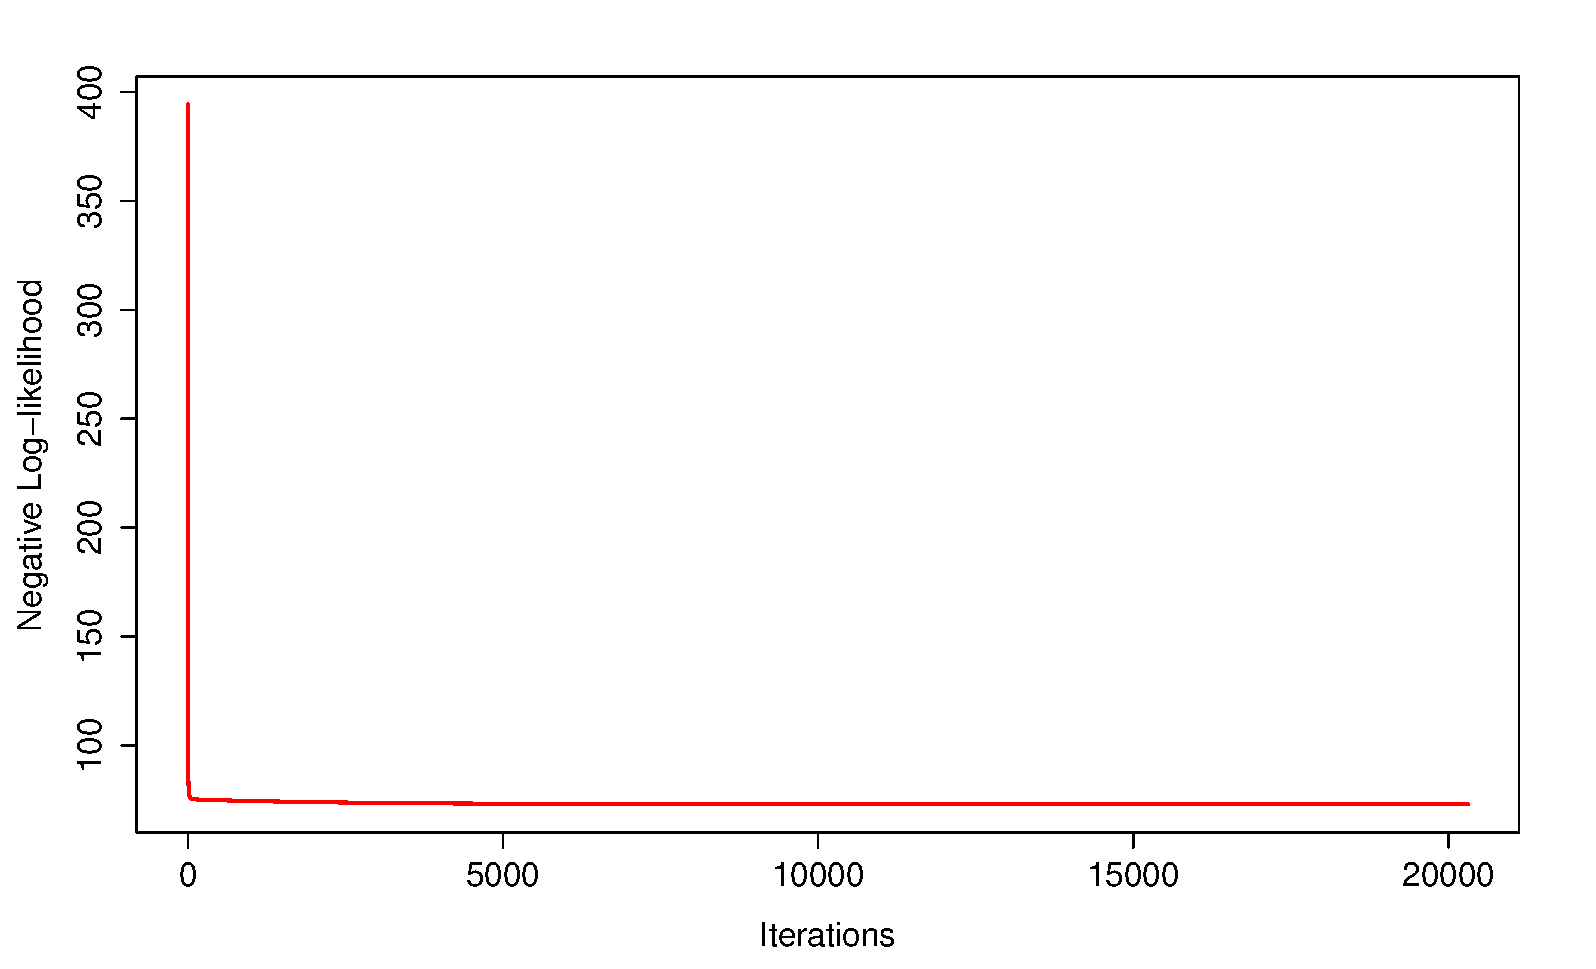
\includegraphics[width=0.6\columnwidth]{./Img/ll}
\caption{Negative log-likelihood of the data as the gradient descent converges.}
\label{fig:grad}
\end{figure}

\item In order to write the second-order Taylor approximation, we first need to compute the Hessian of the negative log-likelihood, that is
\begin{align*}
\nabla^2 l(\beta) &= \nabla \left( - \sum_{i=1}^N x_i (y_i - m_i w_i) \right)
\\
&= \left( \sum_{i=1}^N \nabla (m_i x_{i1} w_i); \dots ; \sum_{i=1}^N \nabla (m_i x_{ip} w_i) \right).
\end{align*}

By exploiting the fact that $\frac{\partial w_i}{\partial \beta_j} = x_{ij} w_i (1 - w_i)$, we obtain, 
\begin{align*}
\nabla^2 l(\beta) &= \left( \begin{array}{ccc}
\sum_{i=1}^N m_i x_{i1} x_{i1} w_i (1 - w_i) & \hdots & \sum_{i=1}^N m_i x_{ip} x_{i1} w_i (1 - w_i) \\ 
\vdots & \ddots & \vdots \\ 
\sum_{i=1}^N m_i x_{i1} x_{ip} w_i (1 - w_i) & \hdots & \sum_{i=1}^N m_i x_{ip} x_{ip} w_i (1 - w_i)
\end{array} 
\right)
\\
&= X^T W X, 
\end{align*}
where the matrix W is defined as $W = \text{diag} \{ m_1 w_1 (1-w_1); \dots ; m_N w_N (1-w_N) \}$. 

The second order Taylor expansion is then 
\begin{align*}
\tilde{l} (\beta) &= l (\beta_0) + \nabla l (\beta_0)^T (\beta - \beta_0) + \frac{1}{2} (\beta - \beta_0)^T \nabla^2 l (\beta_0) (\beta - \beta_0)
\\
&= l (\beta_0) - (y - m w)^T X (\beta - \beta_0) + \frac{1}{2} (\beta - \beta_0)^T X^T W X (\beta - \beta_0)
\\
&= l (\beta_0) - (y-mw)^T X \beta + (y - mw)^T X \beta_0 
\\
&\quad + \frac{1}{2} \beta^T X^T W X \beta + \frac{1}{2} \beta_0^T X^T W X \beta_0 - \beta_0^T X^T W X \beta
\\
&=l (\beta_0) + (y - mw)^T X \beta_0 + \frac{1}{2} \beta_0^T X^T W X \beta_0 
\\
&\quad - (y - mw + WX\beta_0)^T X \beta + \frac{1}{2} (X \beta)^T W (X \beta)
\\
&=\frac{1}{2} ( z - X \beta)^T W ( z - X \beta) + c,
\end{align*}
where 
\begin{align*}
&z = -W^{-1} (y - mw + WX \beta_0) = W^{-1}(mw - y) - X \beta_0;
\\
&c = l(\beta_0) + (y - mw)^T X \beta_0 + \frac{1}{2} \beta_0^T X^T W X \beta_0 
\\
&\quad \text{ } - \frac{1}{2} (y - mw + WX \beta_0)^T W^{-1} (y - mw + WX \beta_0).
\end{align*}

\item Newton's method has successfully been implemented. As a stopping criterion, we used the $L^2$-norm of the difference between two consecutive values of the $\beta$ parameter we are trying to estimate, as before.

We tested the validity of this method on the same real dataset as before. In Figure \ref{fig:newton} the values of the negative log-likelihood are displayed. The gradient descent converges, in this case, after $11$ iterations.

\begin{figure}[!ht]
\centering
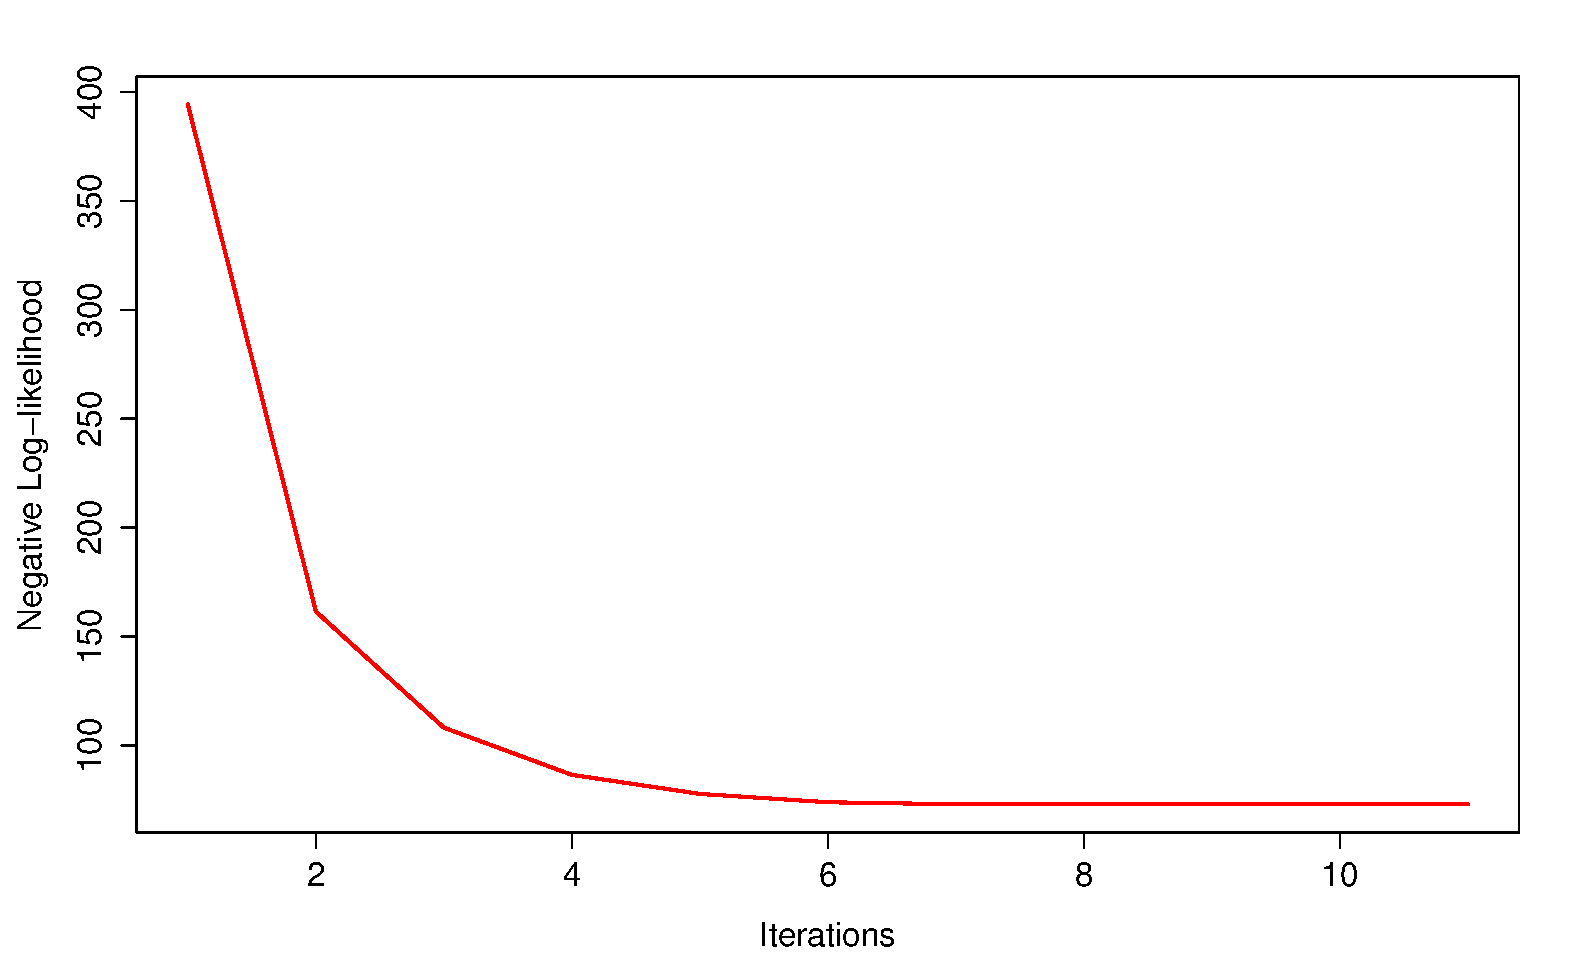
\includegraphics[width=0.6\columnwidth]{./Img/ll_2}
\caption{Negative log-likelihood of the data as Newton's method converges.}
\label{fig:newton}
\end{figure}

\item As we have seen, Newton's method is significantly faster than gradient descent in terms of the total number of iterations that are needed to reach convergence. However, be aware that each iteration of Newton's method is computationally more intense, as it involves the computation of the Hessian matrix and, moreover, the resolution of a linear system. Overall, Newton's method converges more rapidly as it is able to fully exploit the information provided by the second derivatives of the function we are trying to minimize. 

Newton's method is reliable when the difference between the true function and its quadratic approximation is not too large. 


\end{enumerate}


\end{document}
